\documentclass{beamer}
\usepackage{graphicx}
\usepackage{graphics}
\usepackage{hyperref}
\usepackage[english]{babel}
\usepackage[T1]{fontenc}
\usepackage[utf8]{inputenc}
\usepackage{xfrac}
\usepackage{array}


\mode<presentation>
{
    \usetheme{AMUFree-kk}
    \setbeamercovered{transparent = 28}
}
\title{DeepSpeed ZeRO}
\date{2021}
\author{Karol Kaczmarek}
\setbeamertemplate{bibliography item}{[\theenumiv]}


\begin{document}

\begin{frame}
    \titlepage
\end{frame}

\iffalse
\AtBeginSection[]
{
    \begin{frame}
        \frametitle{Outline}
        \tableofcontents[currentsection]
    \end{frame}
}
\fi


\begin{frame}
    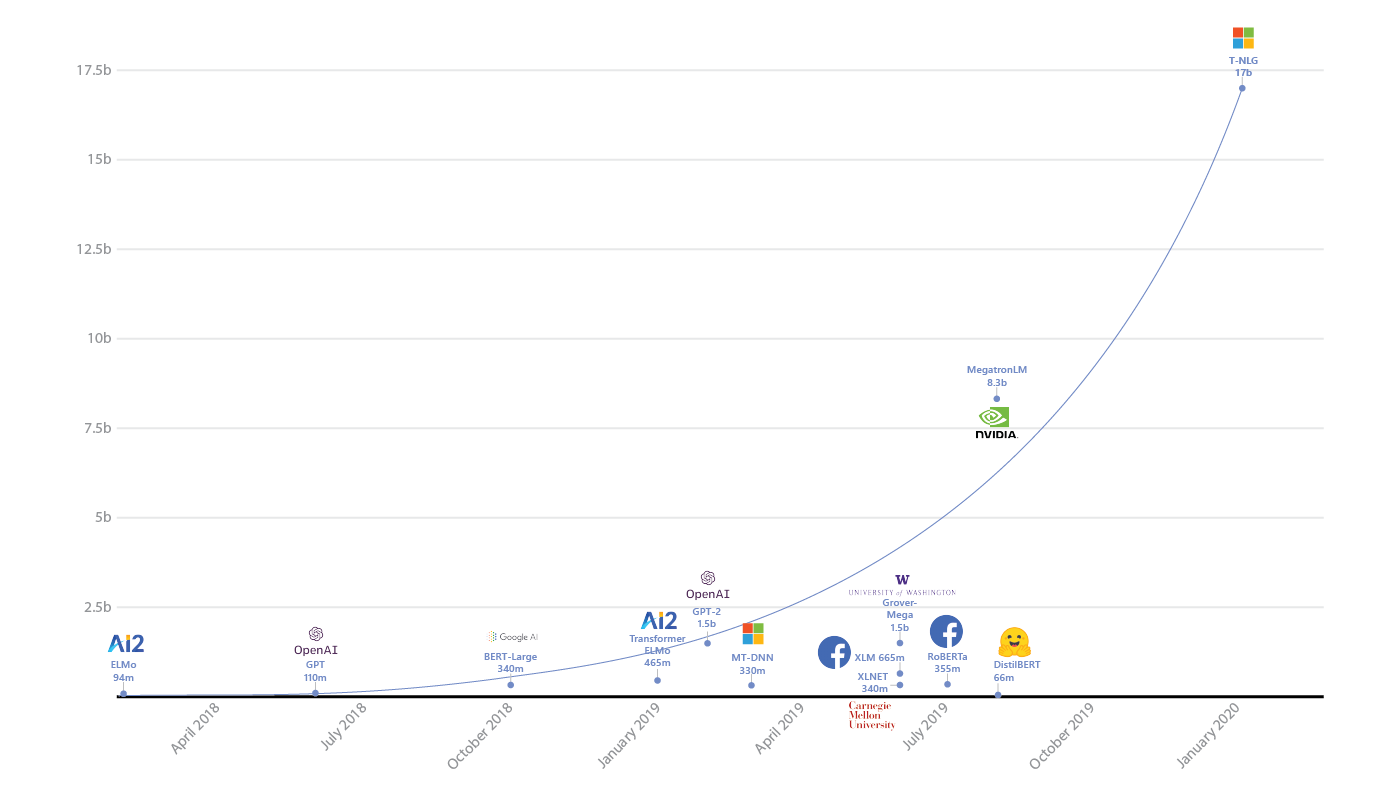
\includegraphics[scale=0.25]{img/TurningNGL.png}
\end{frame}

\begin{frame}
    \frametitle{Data Parallelism (DP)}
    \begin{itemize}
        \item model parameters are replicated on each device
        \item at each step, a mini-batch is divided evenly across all the data parallel processes
        \item each process executes the forward and backward propagation on a different subset of data samples
        \item use of averaged gradients across processes to update the model locally
        \item torch.nn.DataParallel, torch.nn.parallel.DistributedDataParallel
    \end{itemize}
\end{frame}

\begin{frame}
    \frametitle{Model Parallelism (MP)}
    \begin{itemize}
        \item splits the model vertically, partitioning the computation and parameters in each layer across multiple devices
        \item requiring significant communication between each layer
        \item Mesh-Tensorflow \cite{mesh_tensorflow}, Megatron-LM \cite{megatronlm} \cite{megatronlm_2}, L2L \cite{l2l}
    \end{itemize}
\end{frame}


\begin{frame}
    \frametitle{Data Parallelism (DP) and Model Parallelism (MP)}
    \begin{center}
        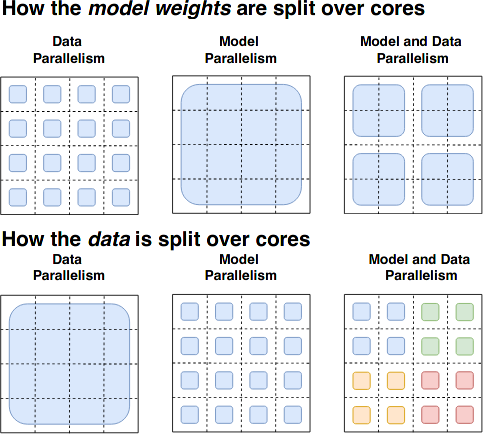
\includegraphics[scale=0.42]{img/data_distribution.png}
    \end{center}
\end{frame}

\begin{frame}
    \frametitle{L2L (layer-to-layer)}
    L2L enables training of networks by keeping one layer/block at a time in GPU memory and only moves tensors in the upcoming layer/block into GPU memory only if needed.
    \begin{center}
        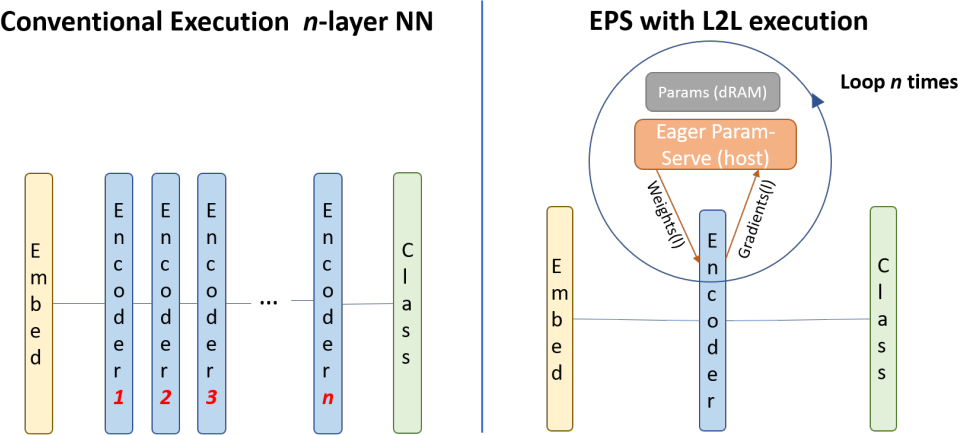
\includegraphics[scale=1.3]{img/L2L.png}

        \tiny{EPS - Eager Param-Server}
    \end{center}
\end{frame}

\begin{frame}
    \frametitle{Pipeline Parallelism (PP)}
    \begin{itemize}
        \item split a model horizontally across layers running each partition on a different device
        \item use micro-batching (part of mini-batch) to hide the pipeline bubble
        \item PipeDream \cite{pipedream}, GPipe \cite{gpipe}, Megatron-LM \cite{megatronlm} \cite{megatronlm_2}
    \end{itemize}
    GPipe:
    \begin{center}
        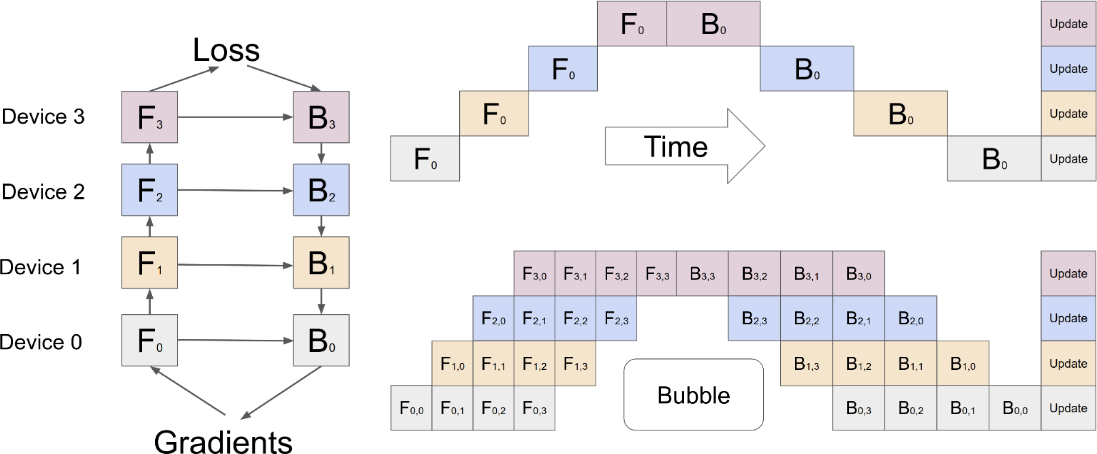
\includegraphics[scale=0.85]{img/gpipe.png}
    \end{center}
\end{frame}

\begin{frame}
    \frametitle{Pipeline Parallelism (PP)}
    Megatron-LM (April 2021) \cite{megatronlm_2} - train 1 trillion parameters  on 3072 GPUs (Nvidia A100 80GB - 384 DGX A100 nodes):
    \begin{center}
        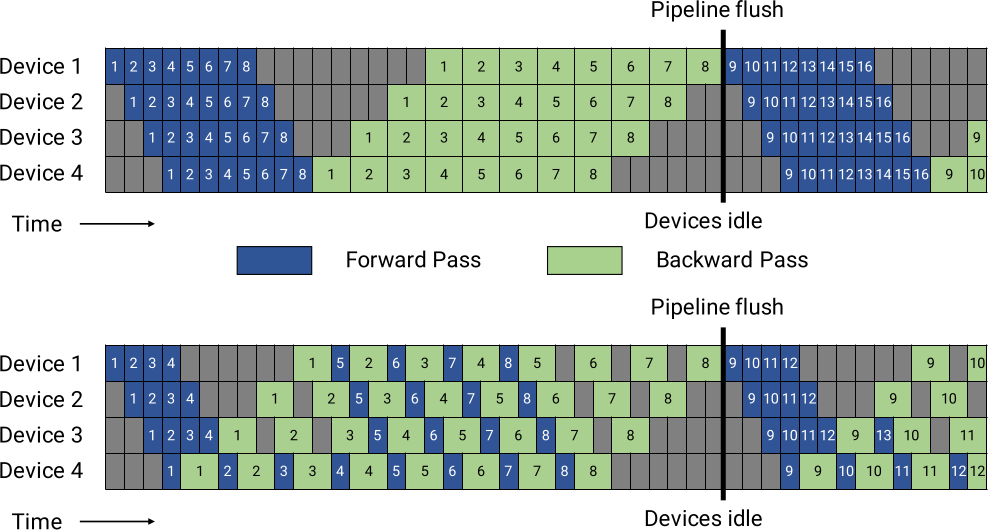
\includegraphics[scale=1.22]{img/megatron_lm.png}
    \end{center}
\end{frame}

\begin{frame}
    \frametitle{Other optimizations}
    \begin{itemize}
        \item \textbf{Activation checkpointing} - reducing the memory footprint of activations - stored from forward pass and reused in backward pass
        \item \textbf{CPU-Offloading} - offloading model states to CPU memory
        \item \textbf{Adaptive optimization} - reducing memory consumption (use other optimizer, like Adafactor)
    \end{itemize}
\end{frame}


% ZeRO
\section{ZeRO}
\begin{frame}
    \frametitle{ZeRO \cite{zero}}
    \begin{itemize}
        \item October 2019 (blogs - February 2020), Microsoft - PyTorch
        \item Turing-NLG - Turing Natural Language Generation - 17B parameters
        \item ZeRO (Zero Redundancy Optimizer) - optimize \textbf{memory}, vastly improving \textbf{training speed} while increasing \textbf{the model size} that can be efficiently trained
        \item runs 100B parameter models on a 400 Nvidia V100 GPU cluster (\textbf{8x} increase in model size and \textbf{10x} increase performance over state-of-the-art - T5 11B)
        \item share ZeRO as a part of our open source DL training optimization library called Deep-Speed - users do not need to modify their model - www.deepspeed.ai
    \end{itemize}
\end{frame}

\begin{frame}
    \frametitle{ZeRO}
    \textbf{ZeRO} has two sets of optimizations:
    \begin{itemize}
        \item \textbf{ZeRO-DP} (ZeRO-powered data parallelism) aimed at reducing the memory footprint of the model states (removes the memory state redundancies across data-parallel processes by \textbf{partitioning} the model states instead of \textbf{replicating})
        \item \textbf{ZeRO-R} targeted towards reducing the residual memory consumption
    \end{itemize}
\end{frame}

\begin{frame}
    \frametitle{ZeRO-DP - Optimizing Model State Memory}
    \textbf{ZeRO-DP} eliminates memory redundancy by partitioning optimizer states ($P_{os}$), gradients ($P_{g}$) and parameters ($P_{p}$) across data parallel processes. \textbf{ZeRO-DP} has three main optimization stages:
    \begin{itemize}
        \item Optimizer State Partitioning ($P_{os}$): $4x$ memory reduction
        \item Add Gradient Partitioning ($P_{os+g}$): $8x$ memory reduction
        \item Add Parameter Partitioning ($P_{os+g+p}$): memory reduction is linear with $N_d$ ($N_d$ = DP degree/data parallelism degree, splitting across $64$ GPUs - $N_d = 64$ will yield a $64x$ memory reduction), modest 50\% increase in communication volume
    \end{itemize}

    With all three stages enabled, ZeRO can train a trillion-parameter model on just 1024 NVIDIA GPUs.
\end{frame}

\begin{frame}
    \frametitle{ZeRO-DP - Comparing stages}
    \begin{center}
        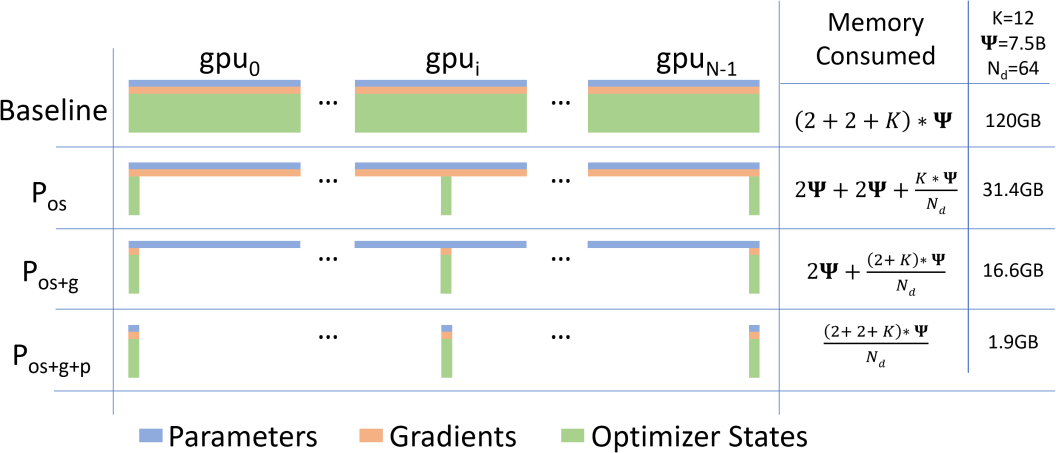
\includegraphics[scale=0.25]{img/zero_memory_consumption.png}
    \end{center}
    \footnotesize{$ K $ - memory multiplier of optimizer states, \textbf{$\psi$} - model size, $N_d$ = DP degree/data parallelism degree}
\end{frame}

\begin{frame}
    \frametitle{ZeRO-DP - Memory consumption}
    \begin{itemize}
        \item ZeRO-1 ($P_{os}$) partitions the optimizer states only
        \item ZeRO-2 ($P_{os+g}$) partitions gradients in addition to optimizer states
        \item ZeRO-3 ($P_{os+g+p}$) partitions all model states
    \end{itemize}
    \begin{center}
        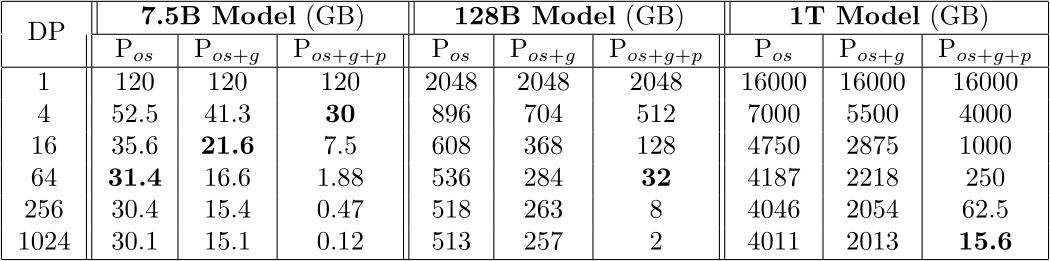
\includegraphics[scale=1.25]{img/zero_memory_consumption_table.png}
    \end{center}
    \tiny{\textbf{Bold-faced text} are the combinations for which the model can fit into a cluster of 32GB V100 GPUs}
\end{frame}

\begin{frame}
    \frametitle{ZeRO-R - Optimizing Residual State Memory}
    The rest of the memory is consumed by  activations, temporary buffers, and unusable memory fragments. \textbf{ZeRO-R} optimize the residual memory consumed by:
    \begin{itemize}
        \item \textbf{activations} (stored from forward pass in order to perform backward pass) - optimize memory by activation partitioning or/and offloads to CPU when appropriate
        \item defines appropriate size for \textbf{temporary buffers} to strike for a balance of memory and computation efficiency
        \item proactively manages memory based on the different lifetime of tensors, preventing \textbf{memory fragmentation}
    \end{itemize}
\end{frame}

\begin{frame}
    \frametitle{ZeRO-R - Residual Memory Consumption}
    Memory consumption for 1.5B parameter GPT-2 model:
    \begin{itemize}
        \item \textbf{Activations} - trained with sequence length of 1K and batch size of 32 requires about 60 GB of memory (proportional to the number of transformer layers $*$ hidden dimensions $*$ sequence length $*$ batch size)
        \item \textbf{Temporary buffers} - fp32 buffer would required 6 GB of memory
        \item \textbf{Memory Fragmentation} - significant memory fragmentation when training very large models, resulting in out of memory issue with over 30\% of memory still available in some extreme cases
    \end{itemize}
\end{frame}

\begin{frame}
    \frametitle{ZeRO training}
    \tiny{Baseline - 384 GPUs, ZeRO - 400 GPUs}
    \begin{center}
        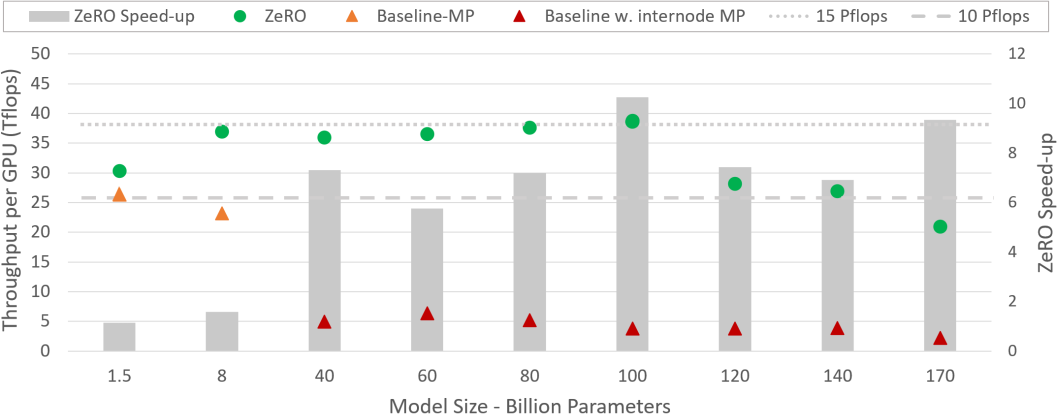
\includegraphics[scale=1.25]{img/zero_model_training_flops.png}
    \end{center}
    \tiny{More in paper: Memory/Communication Analysis, 1 Trillion Parameters, Comparing to Megatron-LM}
\end{frame}


% ZeRO-Offload
\section{ZeRO-Offload}
\begin{frame}
    \frametitle{ZeRO-Offload \cite{zero_offload}}
    \begin{itemize}
        \item January 2021, Microsoft - PyTorch
        \item train models with over 13 billion parameters on a single GPU (Nvidia V100 32GB)
        \item 10x increase size and without model change
        \item offloading data and compute to CPU
        \item designed to minimize the data movement to/from GPU
        \item reduce CPU compute time while maximizing memory savings on GPU
to their existing training pipeline
        \item part of an Open-Source PyTorch library, DeepSpeed - www.deepspeed.ai
        \item does not require model refactoring to work - can enable with few lines of code change
    \end{itemize}
\end{frame}

\begin{frame}
    \frametitle{ZeRO-Offload idea}
    \begin{itemize}
        \item offload the gradients, optimizer states and optimizer computation to CPU, while keeping the parameters and forward and backward computation on GPU
        \item enables a 10x increase in model size, with minimum communication and limited CPU computation
        \item ZeRO-Offload works with ZeRO to scale deep learning training to multiple GPUs - ZeRO-Offload works symbiotically with ZeRO-2
        \begin{itemize}
        	\item \footnotesize{ZeRO: ZeRO-1, ZeRO-2 and ZeRO-3 corresponding to the partitioning of the three different model states, optimizer states, gradients and parameters, respectively}
        \end{itemize}
    \end{itemize}
\end{frame}

\begin{frame}
    \frametitle{ZeRO-Offload idea}
    \begin{itemize}
        \item compute complexity of training per iteration is
generally given by $O(MB)$, where $M$ is the model size and $B$
is the batch size
        \item CPU computation should have a compute complexity lower than $O(MB)$ to avoid bottleneck
        \item forward and backward propagation ($O(MB)$ complexity) should be done on the GPU
        \item remaining computations (norm calculations, weight updates, etc. - $O(M)$ complexity) maybe offloaded and computed to the CPU
    \end{itemize}
\end{frame}

\begin{frame}
    \frametitle{ZeRO-Offload design}
    \begin{itemize}
        \item requires CPU to perform $O(M)$ computation compared to $O(MB)$ on GPU where $M$ and $B$ are the model size and batch sizes
        \item large batch sizes - CPU computation is not a bottleneck
        \item small batch sizes - CPU compute can be a bottleneck
        \item optimization to avoid bottleneck:
        \begin{itemize}
            \item CPU optimizer that is up to 6x faster than the-state-of-art
            \item one-step delayed parameter update (DPU) that allows overlapping the CPU optimizer step with GPU compute
        \end{itemize}
        \item achieves excellent scalability on up to 128 GPUs (near linear speedup)
    \end{itemize}
\end{frame}

\begin{frame}
    \frametitle{ZeRO-Offload dataflow}
    \begin{center}
        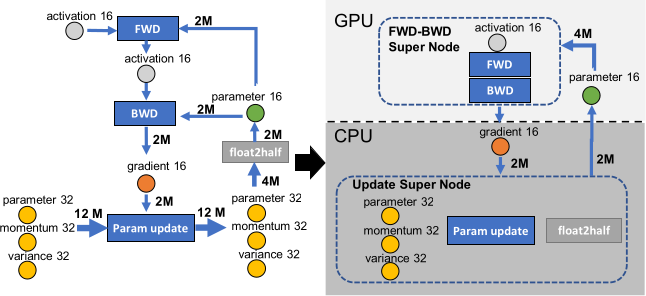
\includegraphics[scale=2.0]{img/zero_offload_dataflow.png}
    \end{center}
    \tiny{$M$ - model parameters, $16$ - fp16, $32$ - fp32}
\end{frame}

\begin{frame}
    \frametitle{ZeRO-Offload training process}
    \footnotesize{Single GPU:}
    \begin{center}
        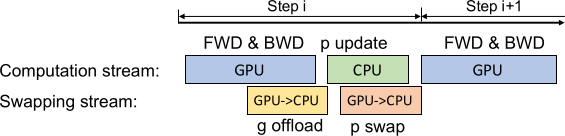
\includegraphics[scale=1.35]{img/zero_offload_single_gpu.png}
    \end{center}
    \footnotesize{Multi GPUs:}
    \begin{center}
        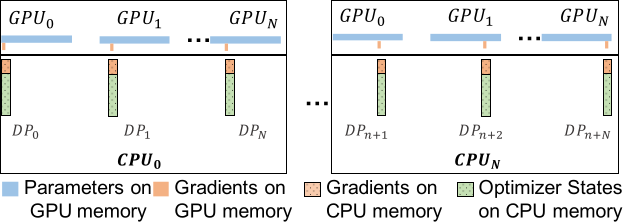
\includegraphics[scale=1.3]{img/zero_offload_multi_gpu.png}
    \end{center}
    \tiny{Total CPU update time decreases with increased data parallelism}
\end{frame}

\begin{frame}
    \frametitle{Fast CPU Adam optimizer}
    \begin{itemize}
        \item SIMD vector instruction (best performance with AVX512 SIMD instruction set) for fully exploiting the hardware parallelism supported on CPU architectures
        \item loop unrolling, an effective technique for increasing instruction level parallelism that is crucial for better memory bandwidth utilization
        \item OMP multithreading for effective utilization of multiple cores and threads on the CPU in parallel
        \item Mixed Precision Training - casting fp16 <-> fp32
    \end{itemize}
\end{frame}

\begin{frame}
    \frametitle{Fast CPU Adam optimizer - latency}
    \begin{center}
        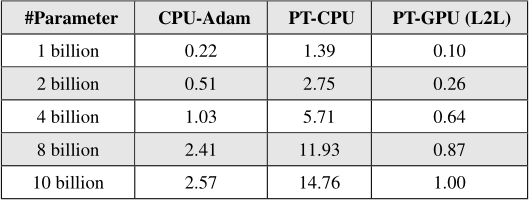
\includegraphics[scale=2.0]{img/adam_latency.png}

        \tiny{PT - PyTorch}
    \end{center}
\end{frame}

\begin{frame}
    \frametitle{One-Step Delayed Parameter Update}
    Delayed Parameter Update (DPU) training schedule:
    \begin{itemize}
        \item first $N - 1$ steps, are trained without DPU to avoid
destabilizing
        \item step $N$, we obtain the gradients from the GPU, but we skip the CPU optimizer step, and do not update the fp16 parameters on the GPU either
        \item step $N + 1$, we compute the parameter updates on the CPU using gradients from step N, while computing the forward and backward pass on the GPU in parallel using parameters updated at step $N - 1$
        \item training with DPU achieves same model training accuracy with higher training throughput
    \end{itemize}
\end{frame}

\begin{frame}
    \frametitle{One-Step Delayed Parameter Update}
    \begin{center}
        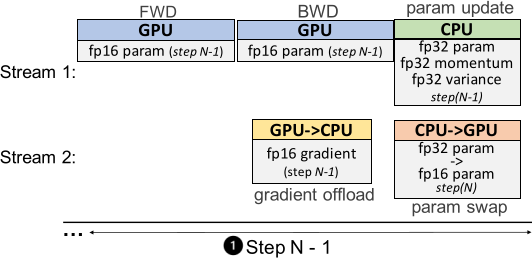
\includegraphics[scale=1.45]{img/delayed_parameter_update_1.png}
    \end{center}
    \begin{center}
        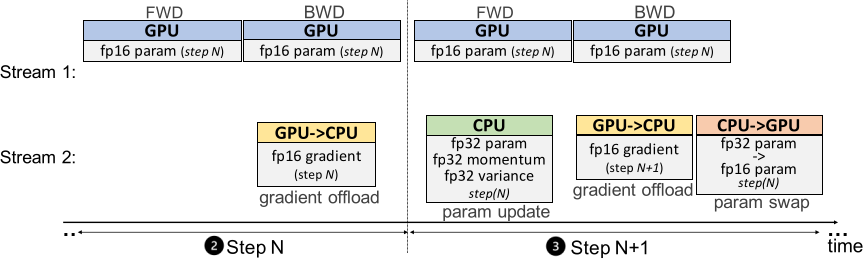
\includegraphics[scale=1.45]{img/delayed_parameter_update_2.png}
    \end{center}
\end{frame}

\begin{frame}
    \frametitle{ZeRO-Offload training results}
    \footnotesize{Train GPT-2 model on single DGX-2 (16 x NVIDIA V100 32GB, CPU Intel Xeon - support AVX512)}:
    \begin{center}
        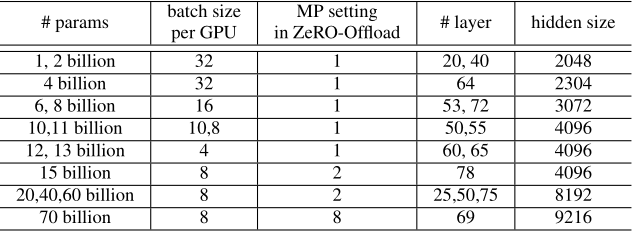
\includegraphics[scale=1.6]{img/zero_offload_gpt2_size.png}
    \end{center}
    \footnotesize{Compared with:}
    \begin{itemize}
        \item \footnotesize{\textbf{PyTorch DDP} - train with} \textbf{DistributedDataParallel}
        \item \footnotesize{\textbf{Megatron-LM} - train up to 8.3B parameter models using 512 GPUs}
        \item \footnotesize{\textbf{L2L} - keeping one Transformer block at a time in GPU}
        \item \footnotesize{\textbf{ZeRO} - extends data parallelism with memory redundancies}
    \end{itemize}
    .
\end{frame}

\begin{frame}
    \frametitle{ZeRO-Offload training results}
    \begin{center}
        \begin{tabular}{ l l }
        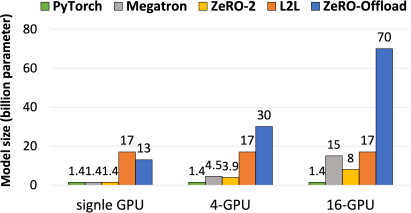
\includegraphics[scale=1.5]{img/zero_offload_single_gpu_size.png}
        & 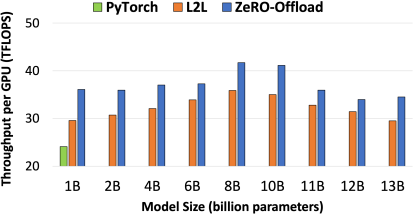
\includegraphics[scale=1.5]{img/zero_offload_single_gpu_batch512.png}\\
        \tiny{The size of the biggest model that can be trained} & \tiny{The training on a single GPU with a batch size of 512}
        \end{tabular}
    \end{center}
    \begin{itemize}
        \item ZeRO-Offload - 13B on a single GPU (9x larger than using PyTorch,
Megatron, and ZeRO-2)
        \item ZeRO-Offload increases the model size by 50x (PyTorch), 4.5x (Megatron), 7.8x (ZeRO-2) and 4.2x (L2L) on 16 GPUs
    \end{itemize}
\end{frame}

\begin{frame}
    \frametitle{ZeRO-Offload with/without DPU}
    The training throughput is compared for w/o DPU and w/ DPU to GPT-2. Batch size is set to 8.
    \begin{center}
        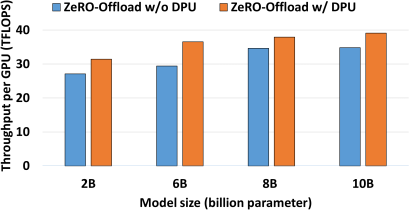
\includegraphics[scale=2.0]{img/zero_offload_dpu.png}
    \end{center}
\end{frame}

\begin{frame}
    \frametitle{ZeRO-Offload with model parallelism}
    \begin{center}
        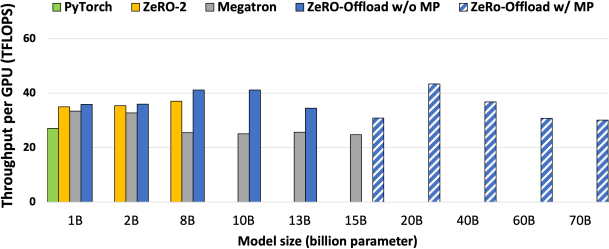
\includegraphics[scale=2.0]{img/zero_offload_max_model.png}
    \end{center}
\end{frame}

\begin{frame}
    \frametitle{ZeRO-Offload scalability}
    Comparison of training throughput between ZeRO-Offload and ZeRO-2 using 1-128 GPUs for a 10B parameter GPT2
    \begin{center}
        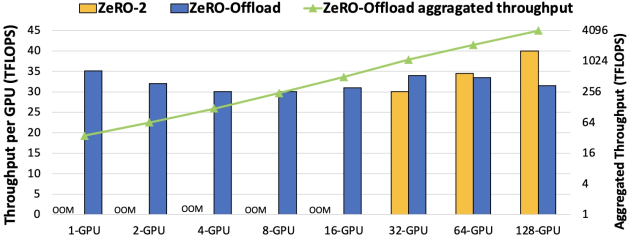
\includegraphics[scale=2.0]{img/zero_offload_scalability.png}
    \end{center}
\end{frame}




% ZeRO-Infinity
\section{ZeRO-Infinity}
\begin{frame}
    \frametitle{ZeRO-Infinity \cite{zero_infinity}}
    \begin{itemize}
        \item April 2021, Microsoft - PyTorch
        \item \textbf{ZeRO-Infinity} - heterogeneous system technology that leverages GPU, CPU, and NVMe memory to allow for unprecedented model scale on limited resources without requiring model code refactoring
        \item available through DeepSpeed (ZeRO-Infinity extends the ZeRO with new innovations in heterogeneous memory access called the \textbf{infinity offload engine})
        \item running 32 trillion parameters on 32 NVIDIA DGX-2 nodes (512 V100 GPUs)
        \item supports 1 trillion parameters per NVIDIA V100 DGX-2 node - 50x increase over 3D parallelism
    \end{itemize}
\end{frame}

\begin{frame}
    \frametitle{Memory/Bandwidth requirements \footnotesize{(more analysis in paper})}
    \begin{center}
        \footnotesize{Memory requirements for models:}
        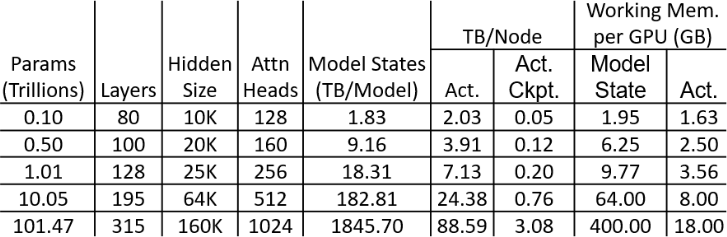
\includegraphics[scale=1.35]{img/zero_infinity_mem_requirements.png}
    \end{center}
    \begin{center}
        \footnotesize{Available memory and achievable bandwidth (NVIDIA V100
DGX-2 Cluster):}
        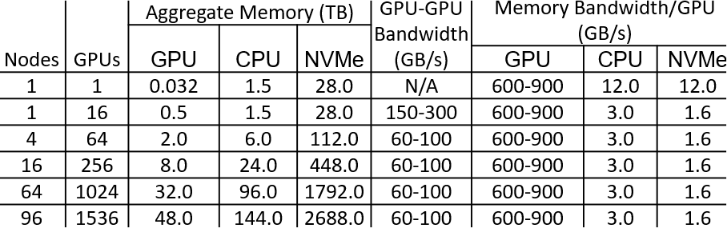
\includegraphics[scale=1.35]{img/zero_infinity_mem_available.png}
    \end{center}
\end{frame}

\begin{frame}
    \frametitle{ZeRO-Infinity}
    \textbf{ZeRO-Infinity} consisting five technologies:
    \begin{itemize}
        \item \textbf{infinity offload engine} - fully leverage heterogeneous architecture on modern clusters by simultaneously exploiting GPU, CPU and NVMe memory, and GPU and CPU compute
        \item \textbf{memory-centric tiling} - handle massive operators without requiring model parallelism
        \item \textbf{bandwidth-centric partitioning} - leveraging aggregate memory bandwidth across all parallel devices
        \item \textbf{overlap-centric design} - overlapping compute and communication
        \item \textbf{ease-inspired implementation} - avoid model code refactoring
    \end{itemize}
\end{frame}

\begin{frame}
    \frametitle{Design for unprecedented scale}
    \textbf{NVMe} storage that is over \textbf{50x} larger than the GPU memory and nearly \textbf{20x} larger than CPU memory.
    \begin{itemize}
        \item \textbf{Infinity offload engine for model states} - built on top of ZeRO-3 which partitions all model states to remove memory redundancy refactoring (DeepNVMe - C++ NVMe read/write library - capable of achieving near peak read and write bandwidths on the NVMe)
        \item \textbf{CPU Offload for activations} - offload activation memory to CPU memory, when necessary (0.76 TB for 10 trillion parameter model)
        \item \textbf{Memory-centric tiling for working memory} - breaking down a large operator into smaller tiles that can be executed sequentially (automatically)
    \end{itemize}
\end{frame}

\begin{frame}
    \frametitle{Design for excellent training efficiency}
    \begin{itemize}
        \item \textbf{bandwidth-centric partitioning} - data mapping and parallel data retrieval strategy for offloaded parameters and gradients that allows ZeRO-Infinity to achieve virtually unlimited heterogeneous memory bandwidth (using \textbf{allgather} instead of a \textbf{broadcast} when a parameter needs to be accessed)
        \item \textbf{overlap centric design} - allows to overlap not only GPU-GPU communication with computation but also NVMe-CPU and CPU-GPU communications (traces the forward and backward computation on that fly and prefetches the parameter requires by the future operators)
    \end{itemize}
\end{frame}

\begin{frame}
    \frametitle{Design for ease of use}
    Eliminates the need for manual model code refactoring even when scaling to trillions of parameters.

    \textbf{Ease-inspired implementation} with two automated features:
    \begin{itemize}
        \item \textbf{automated data movement} - gather and partition parameters right before and after they are required during the training (pre/post forward/backward hooks into PyTorch submodules)
        \item \textbf{automated model partitioning during initialization} - wrapping the constructor of all module classes so that parameters of each submodule are partitioned and offloaded immediately
    \end{itemize}
\end{frame}

\begin{frame}
    \frametitle{Training overview}
    \begin{center}
        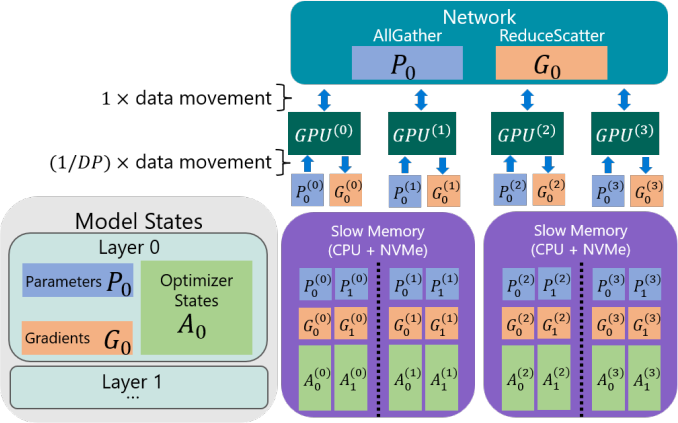
\includegraphics[scale=1.3]{img/zero_infinity_overview.png}
    \end{center}
    \begin{itemize}
    	\tiny{\item model with two layers on four data parallel (DP) ranks}
    	\tiny{\item partitioned parameters ($P_n$) are moved from slow memory to GPU and then collected to form the full layer}
    	\tiny{\item after gradients are computed, they are aggregated, repartitoned, and then offloaded to slow memory}
    	\tiny{\item $P_0^{(2)}$ is the portion of $0$-layer parameters owned by $GPU^{(2)}$}
    \end{itemize}
\end{frame}

\begin{frame}
    \frametitle{Efficiently training}
    \begin{center}
        \begin{tabular}{ c c }
        \tiny{(1)} & \tiny{(2)}\\
        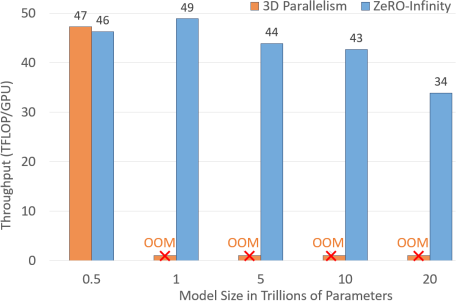
\includegraphics[scale=1.4]{img/zero_infinity_efficiently_trains.png}
        & 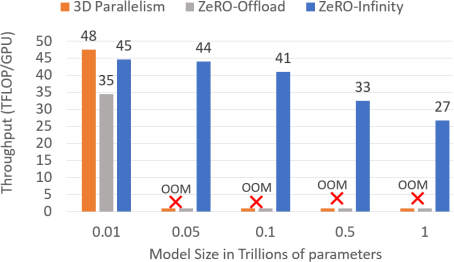
\includegraphics[scale=1.4]{img/zero_infinity_one_trillion.png}
        \end{tabular}
        \begin{enumerate}
        	\tiny{\item ZeRO-Infinity efficiently trains 40x larger models than 3D parallelism on 512 GPUs}
        	\tiny{\item ZeRO-Infinity can train up to 1T model on a DGX-2 node (16 GPUs) without model parallelism}
        \end{enumerate}
    \end{center}
\end{frame}

\begin{frame}
    \frametitle{\normalsize{Different device placement and partitioning strategies}}
    \begin{center}
        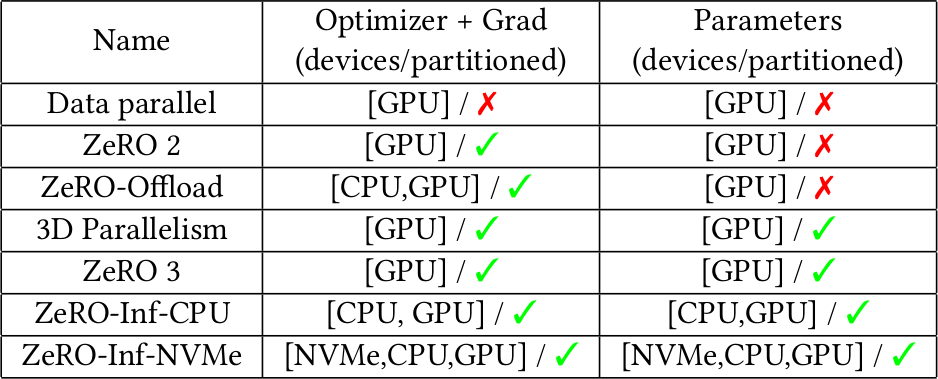
\includegraphics[scale=1.0]{img/zero_infinity_table_compare.png}
    \end{center}
    \begin{center}
        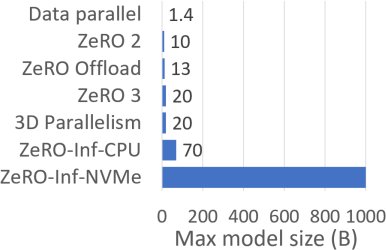
\includegraphics[scale=1.3]{img/zero_infinity_max_model.png}
    \end{center}
\end{frame}

\begin{frame}
    \frametitle{Impact of system features}
    \begin{center}
        \begin{tabular}{ c c }
        \tiny{(1)} & \tiny{(2)}\\
        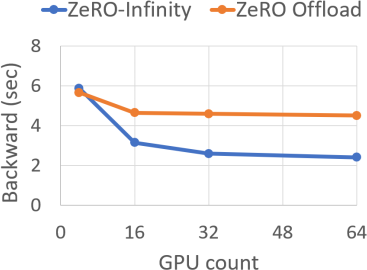
\includegraphics[scale=1.2]{img/zero_infinity_backward_time.png}
        & 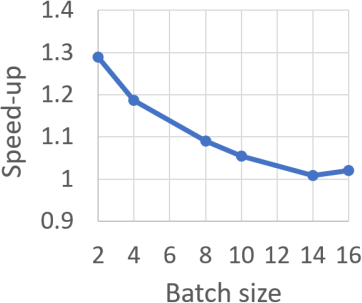
\includegraphics[scale=1.2]{img/zero_infinity_batch_size.png}
        \end{tabular}
        \begin{enumerate}
        	\tiny{\item ZeRO-Infinity speedup of nearly 2x at 64 GPUs compared to ZeRO-Offload}
        	\tiny{\item \textbf{Prefetching} and \textbf{overlapping} are crucial to achieving good performance at small batch sizes per GPU - 8B parameter model with 64 GPUs}
        \end{enumerate}
    \end{center}
    \tiny{More analysis in paper}
\end{frame}


% DeepSpeed
\section{DeepSpeed}
\begin{frame}
    \frametitle{DeepSpeed}
    \begin{itemize}
        \item DeepSpeed
        \begin{itemize}
 			\item \footnotesize{works best with fp16 and Fused Adam/DeepSpeed CPU-Adam}
        	\item \footnotesize{\url{https://www.deepspeed.ai}}
        \end{itemize}
        \begin{center}
    		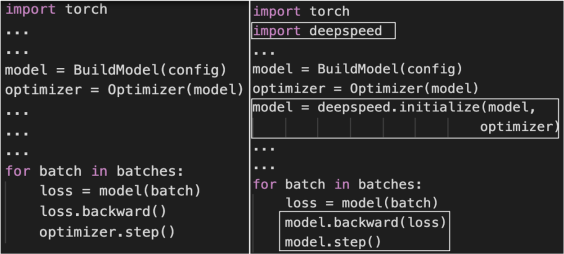
\includegraphics[scale=1.0]{img/deepspeed_zero.png}
	    \end{center}

        \item DeepSpeed with PyTorch Lightning
        \begin{itemize}
        	\item \footnotesize{\url{https://pytorch-lightning.readthedocs.io/en/stable/advanced/advanced_gpu.html?highlight=DeepSpeed\#deepspeed}}
        \end{itemize}

        \item DeepSpeed with transformers trainer
        \begin{itemize}
        	\item \footnotesize{\url{https://huggingface.co/transformers/main_classes/trainer.html}}
        \end{itemize}
    \end{itemize}
\end{frame}


% References
\section{References}
\begin{frame}[allowframebreaks,t]
    \tiny
    \frametitle{References}
    \bibliographystyle{ieeetr}
    \bibliography{zero}
    %\nocite{*}
\end{frame}

\end{document}
